\section{Analysis of the \texttt{q} file}

The analysis of the \texttt{DQD\_SiMOS\_q.vtu} output was carried out in
ParaView by cutting the device at the height of the quantum layer
(\(z=45\,\mathrm{nm}\)) and by extracting a \textit{Plot Over Line} along the
axis connecting the two dots (\(y=136.5\,\mathrm{nm}\)). The plotted quantities
are the confinement potential and the probability densities \(|\psi_i|^2\) of
the first five single-particle eigenstates.

\begin{table}[H]
\centering
\begin{tabular}{c c p{8.2cm}}
\hline
State & Energy [eV] & Localization observed in the quantum slice \\
\hline
Ground & 0.01115999 & Ground orbital of the right dot. \\
1st excited & 0.01120989 & Ground orbital of the left dot. \\
2nd excited & 0.01396172 & First excited orbital of the right dot. \\
3rd excited & 0.01400675 & First excited orbital of the left dot. \\
4th excited & 0.01438458 & Higher orbital with finite density in the barrier region. \\
\hline
\end{tabular}
\caption{First five eigenenergies obtained from the Schr\"odinger solution.}
\label{tab:q-energies}
\end{table}

For an ideal symmetric double dot, the two states belonging to the same
orbital shell should be degenerate. In the simulation they instead appear as
two close but resolved pairs. The ground-state pair is split by
\(4.99\times10^{-5}\,\mathrm{eV}=49.9\,\mu\mathrm{eV}\), while the first
excited pair is split by
\(4.50\times10^{-5}\,\mathrm{eV}=45.0\,\mu\mathrm{eV}\). These splittings are
small compared with the energy separation between the two shells,
\(E_2-E_0\simeq2.80\,\mathrm{meV}\). We therefore interpret the spectrum as
two almost degenerate dot orbitals, staggered by a small left-right asymmetry.
This staggering is already present at the level of the initial geometry/mesh,
so it is reported as a numerical/geometrical splitting of the nominally
degenerate states rather than as an additional physical conclusion from the
post-processing.

\begin{figure}[H]
    \centering
    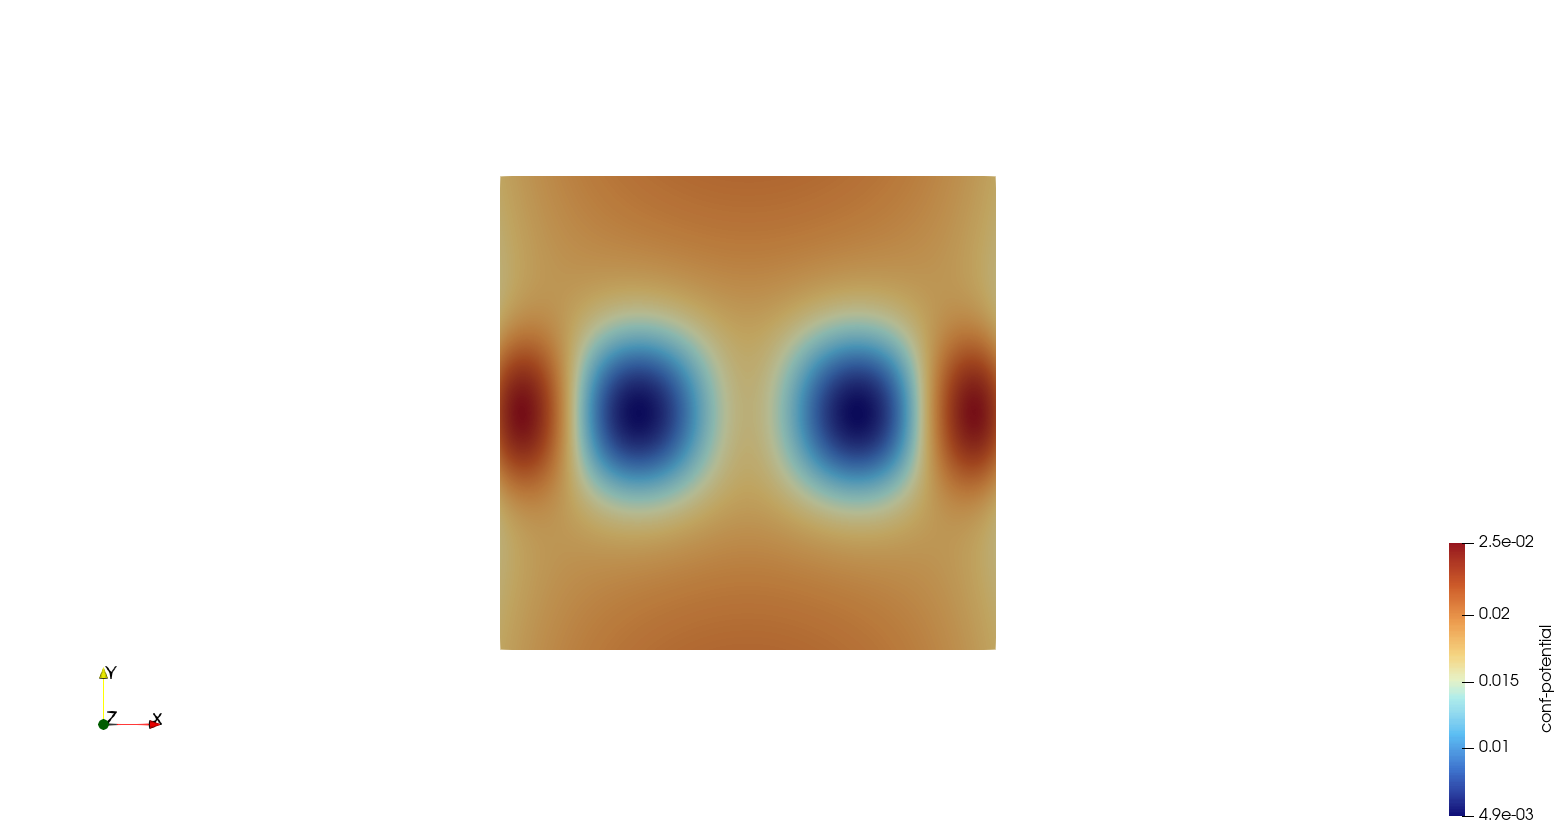
\includegraphics[width=0.72\textwidth]{Images/Qfile/Slice/ConfPotentialSlice.png}
    \caption{Confinement potential on the quantum slice. The two minima define
    the two dots, while the central saddle gives the tunnel barrier.}
    \label{fig:q-conf-slice}
\end{figure}

The confinement map in Fig.~\ref{fig:q-conf-slice} shows two electrostatic
minima separated by a finite central barrier. Sampling the same line used for
the wavefunction plots gives \(V_L\simeq5.03\,\mathrm{meV}\) and
\(V_R\simeq4.84\,\mathrm{meV}\) for the two dot minima, and an inter-dot saddle
of \(V_b\simeq15.83\,\mathrm{meV}\). The fourth excited level,
\(E_4=14.38\,\mathrm{meV}\), is therefore only about \(1.45\,\mathrm{meV}\)
below the barrier top. This explains why this state has a visible probability
density inside the barrier region, while the lower levels remain more strongly
confined inside the individual wells.

\begin{figure}[H]
    \centering
    \begin{subfigure}{0.49\textwidth}
        \centering
        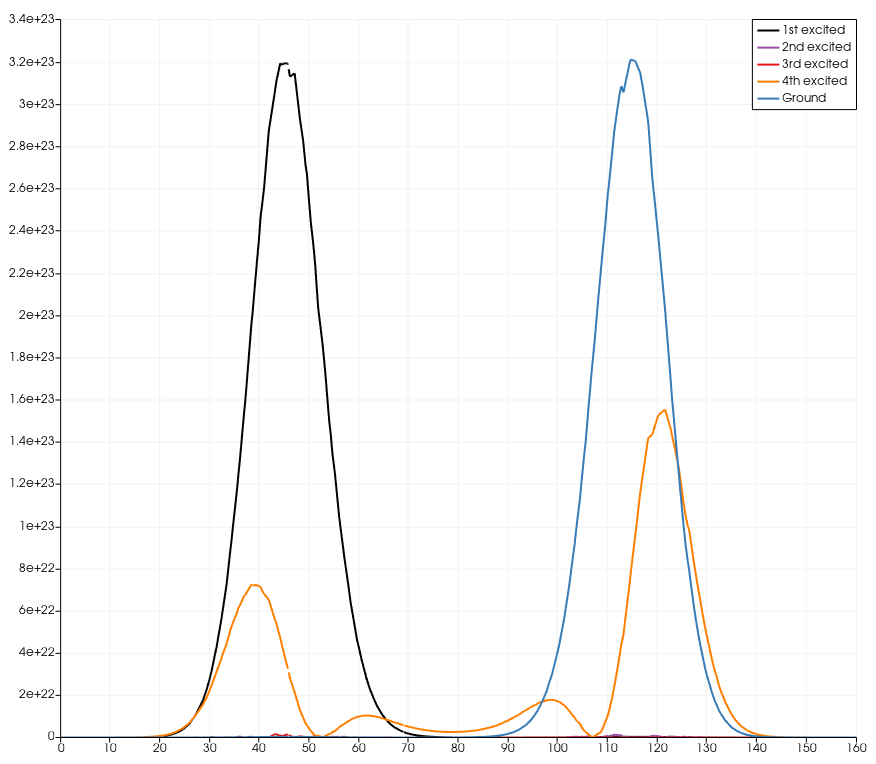
\includegraphics[width=\textwidth]{Images/Qfile/Plots/FullGraph2.png}
        \caption{Linear scale.}
        \label{fig:q-full-linear}
    \end{subfigure}
    \hfill
    \begin{subfigure}{0.49\textwidth}
        \centering
        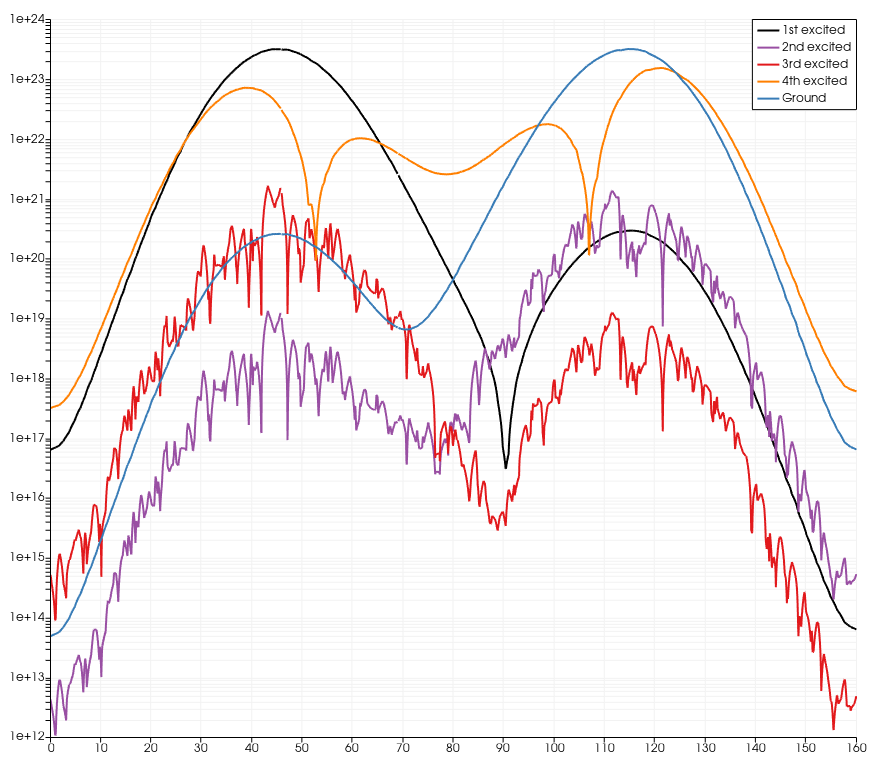
\includegraphics[width=\textwidth]{Images/Qfile/Plots/FullGraphLogNoConf.png}
        \caption{Logarithmic scale.}
        \label{fig:q-full-log}
    \end{subfigure}
    \caption{Probability densities along the axis connecting the two dots. The
    logarithmic representation is more informative because it resolves the
    weak tails and the small excited-state densities that are hidden on the
    linear scale.}
    \label{fig:q-full-graphs}
\end{figure}

The line profiles in Fig.~\ref{fig:q-full-graphs} show the hierarchy of the
states. On the linear scale the two lowest orbitals dominate because their
peak densities are approximately two orders of magnitude larger than the
second and third excited states along the selected line. The logarithmic plot
keeps the same spatial information but makes the lower-amplitude components
visible, in particular the tails across the inter-dot region.

\begin{figure}[H]
    \centering
    \begin{subfigure}{0.32\textwidth}
        \centering
        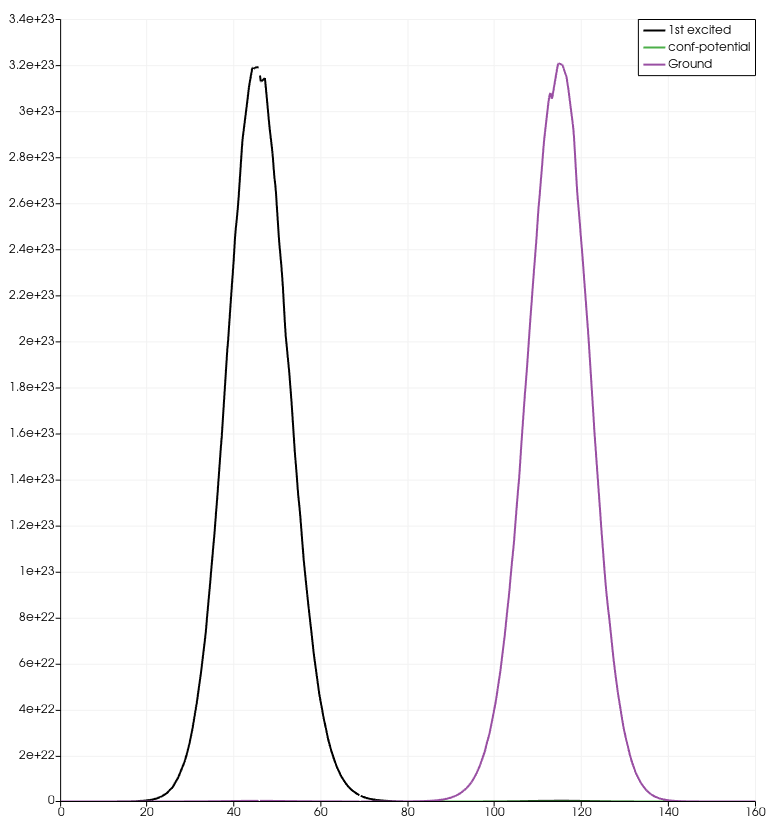
\includegraphics[width=\textwidth]{Images/Qfile/Plots/GroundFirst.png}
        \caption{Ground-state pair.}
        \label{fig:q-ground-first}
    \end{subfigure}
    \hfill
    \begin{subfigure}{0.32\textwidth}
        \centering
        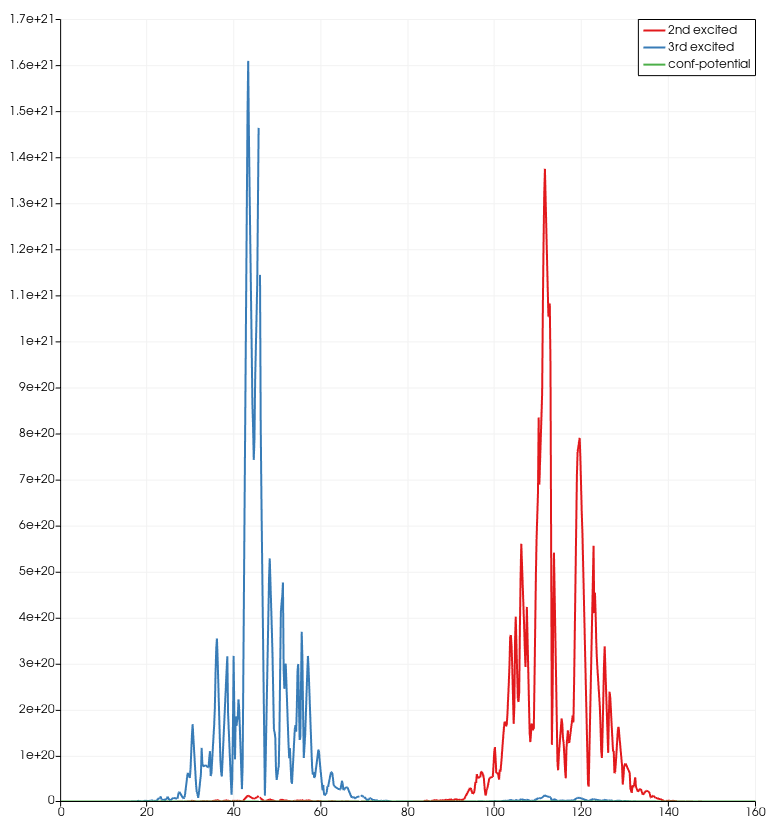
\includegraphics[width=\textwidth]{Images/Qfile/Plots/SecondThird.png}
        \caption{First excited pair.}
        \label{fig:q-second-third}
    \end{subfigure}
    \hfill
    \begin{subfigure}{0.32\textwidth}
        \centering
        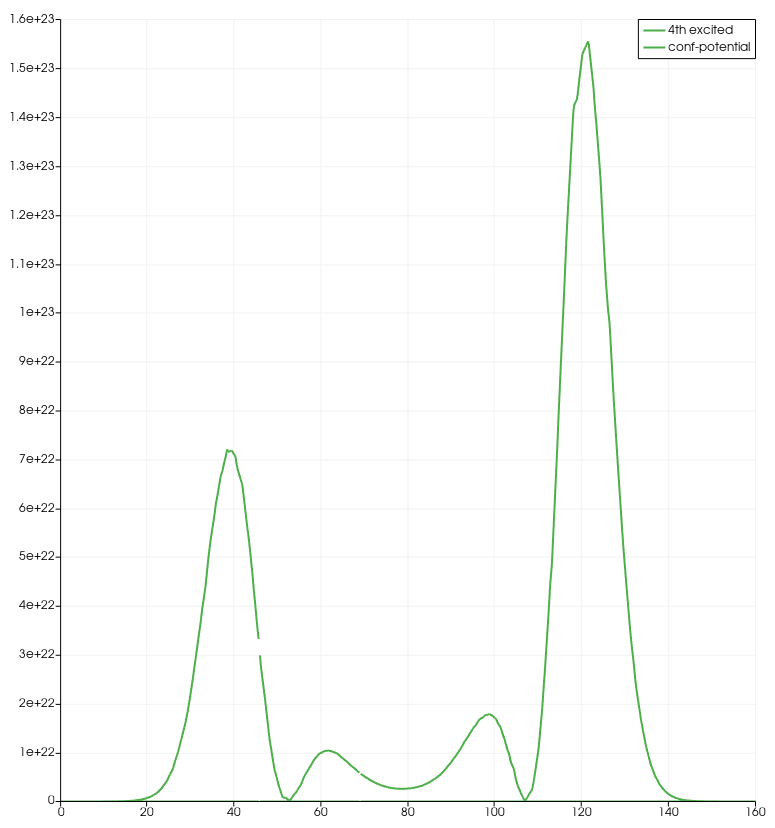
\includegraphics[width=\textwidth]{Images/Qfile/Plots/Fourth.png}
        \caption{Fourth excited level.}
        \label{fig:q-fourth-plot}
    \end{subfigure}
    \caption{Separate line plots for the two quasi-degenerate pairs and for the
    fourth excited state.}
    \label{fig:q-line-plots}
\end{figure}

Figure~\ref{fig:q-line-plots} separates the same spectrum into physically
corresponding groups. The first pair represents the lowest orbital localized
in the two dots, while the second pair represents the first excited orbital in
the two dots. The fourth excited state is different: its profile contains
weight in both wells and in the central barrier. Since its energy is close to
the barrier saddle, this state is the first one showing a clear molecular-like
hybridization between the dots.

\begin{figure}[H]
    \centering
    \begin{subfigure}{0.32\textwidth}
        \centering
        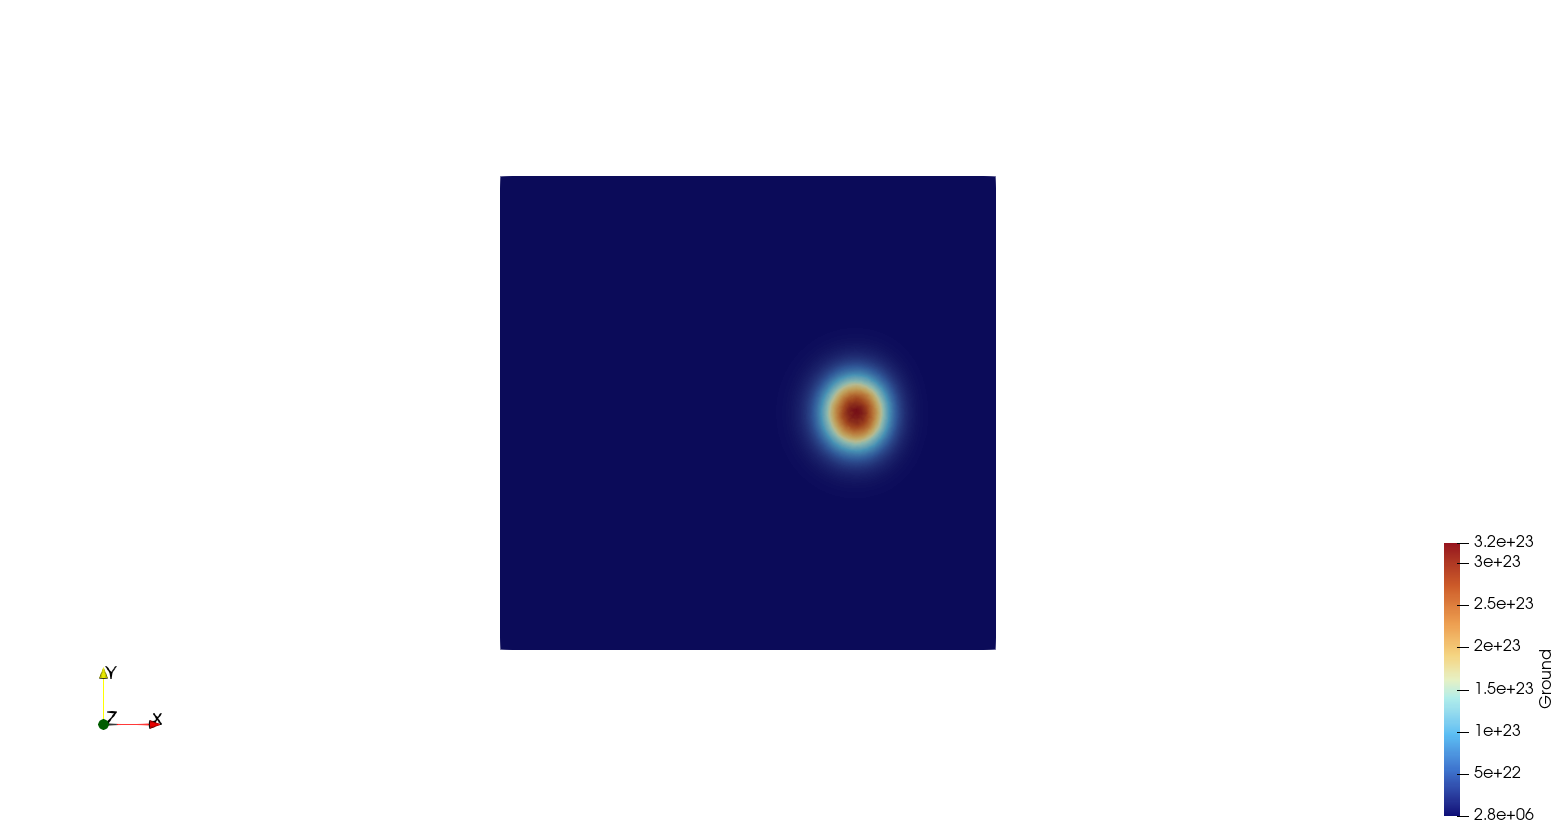
\includegraphics[width=\textwidth]{Images/Qfile/Slice/GroundSlice.png}
        \caption{Ground state.}
    \end{subfigure}
    \hfill
    \begin{subfigure}{0.32\textwidth}
        \centering
        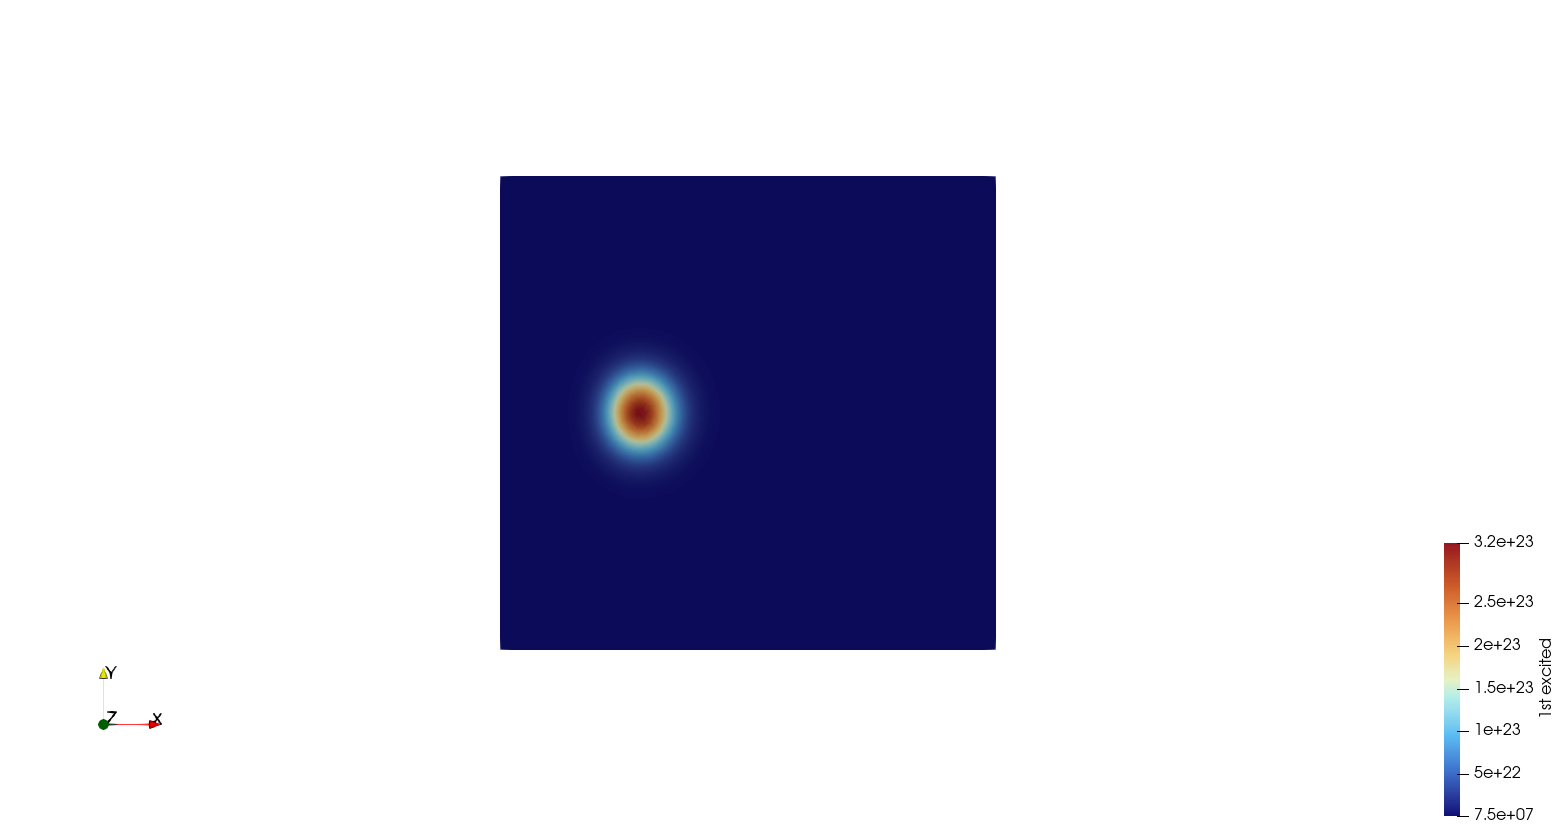
\includegraphics[width=\textwidth]{Images/Qfile/Slice/FirstSlice.png}
        \caption{1st excited state.}
    \end{subfigure}
    \hfill
    \begin{subfigure}{0.32\textwidth}
        \centering
        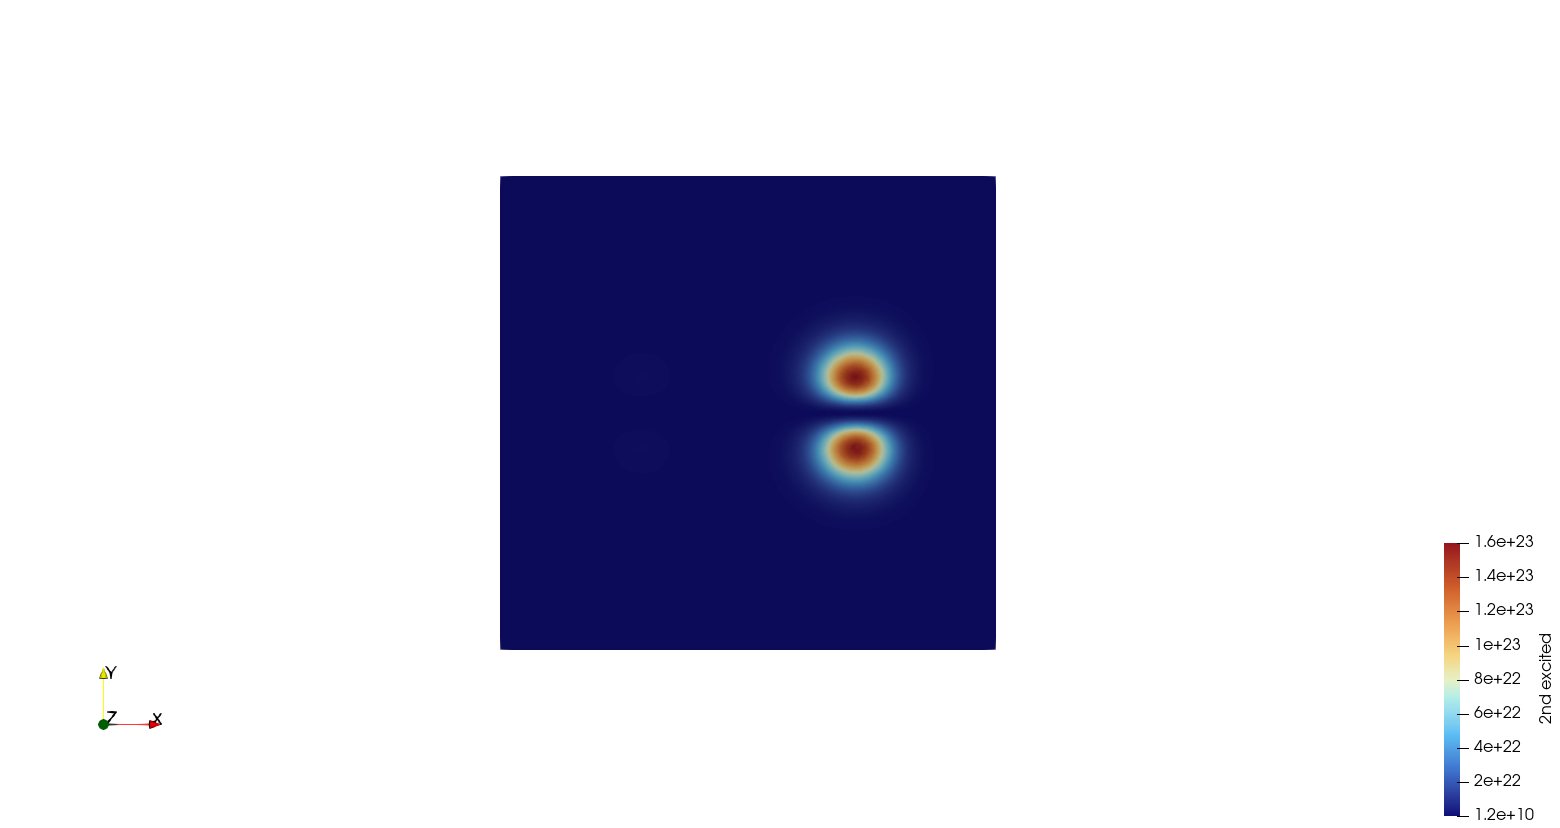
\includegraphics[width=\textwidth]{Images/Qfile/Slice/SecondSlice.png}
        \caption{2nd excited state.}
    \end{subfigure}

    \vspace{0.2cm}

    \begin{subfigure}{0.32\textwidth}
        \centering
        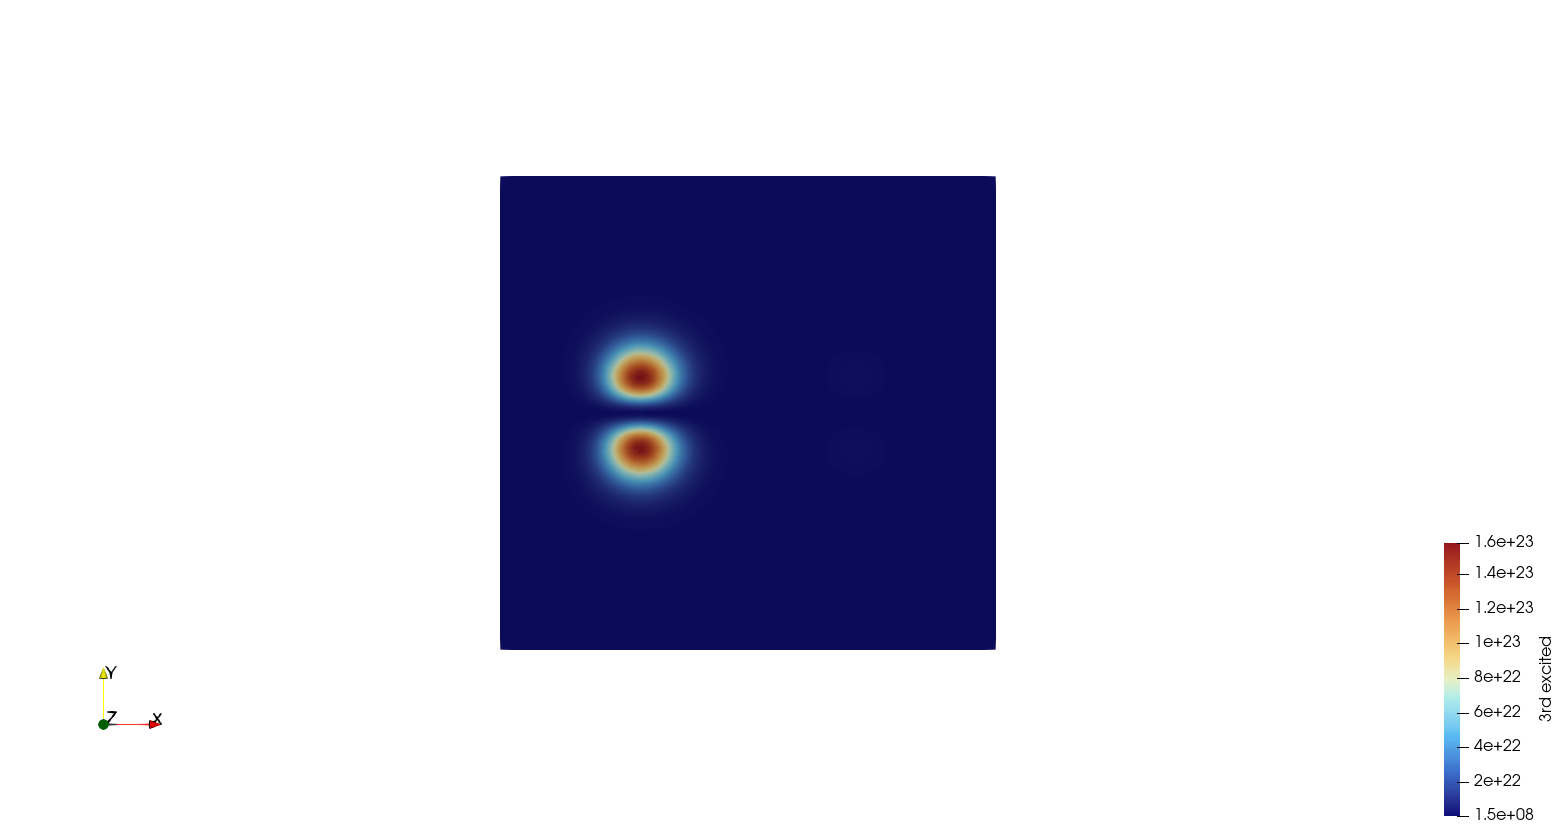
\includegraphics[width=\textwidth]{Images/Qfile/Slice/ThirdSlice.png}
        \caption{3rd excited state.}
    \end{subfigure}
    \hfill
    \begin{subfigure}{0.32\textwidth}
        \centering
        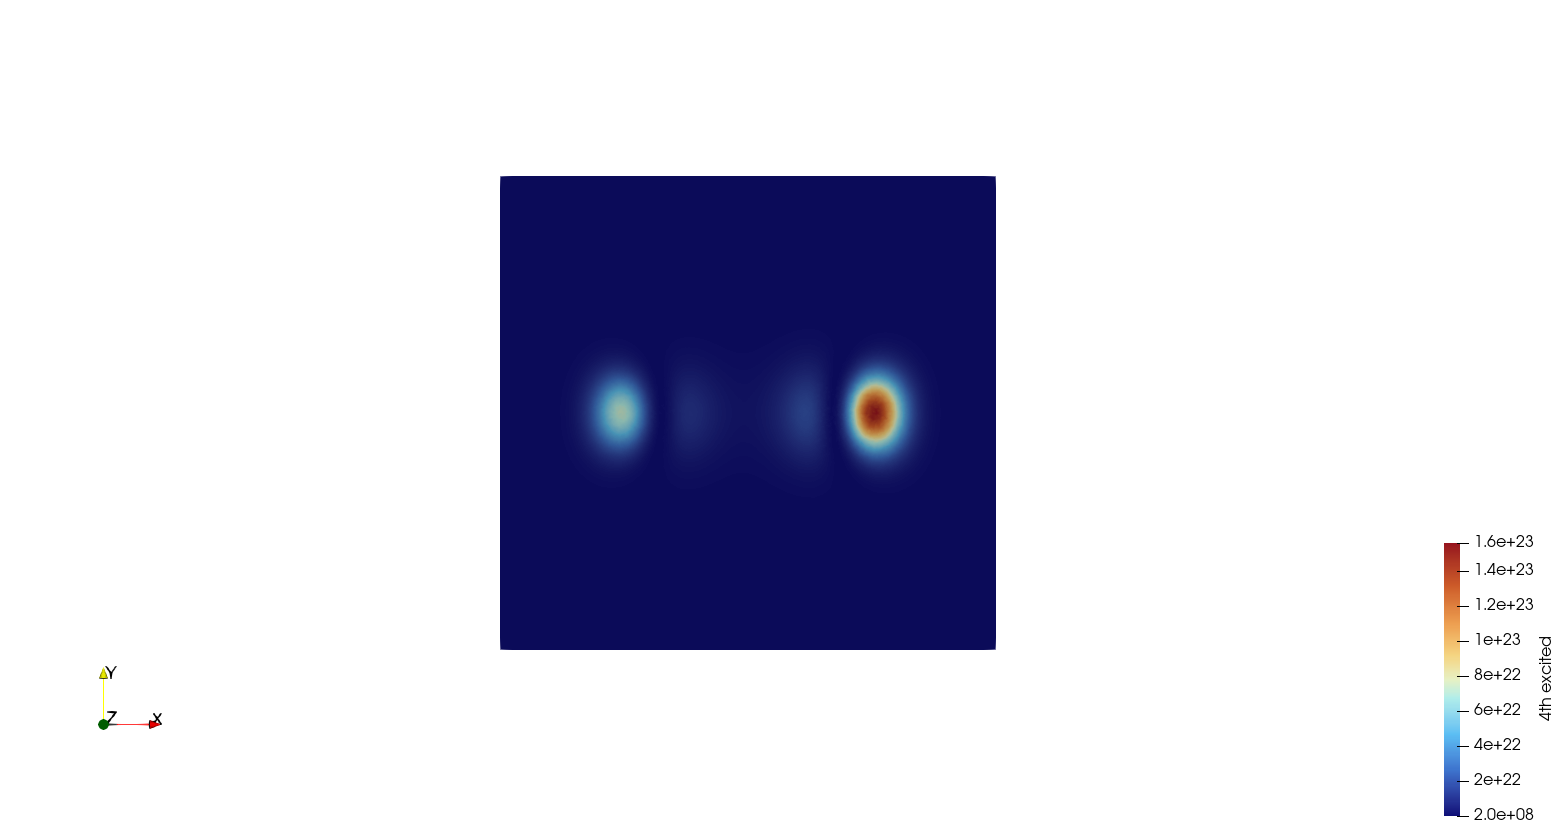
\includegraphics[width=\textwidth]{Images/Qfile/Slice/FourthSlice.png}
        \caption{4th excited state.}
    \end{subfigure}
    \caption{Slices of the probability densities \(|\psi_i|^2\) in the
    quantum region.}
    \label{fig:q-density-slices}
\end{figure}

The density slices in Fig.~\ref{fig:q-density-slices} confirm the assignment
of the line profiles. The two lowest states are single-lobe states localized
in opposite wells. The second and third excited states show the expected
two-lobe structure of the first excited orbital, again localized mainly on one
dot at a time. The fourth excited state is the only one among the computed
levels with an appreciable density in the region separating the two wells.

The device therefore forms the expected double quantum dot: two confined
potential minima, two nearly degenerate orbital pairs, and a finite inter-dot
barrier. The lowest states correspond to a weakly coupled regime, because they
are mostly localized on individual dots. The fourth state instead has a
bonding-like hybridized character, evidenced by the probability density in the
barrier region and by its energy lying close to the barrier saddle.
